\vspace*{4mm}
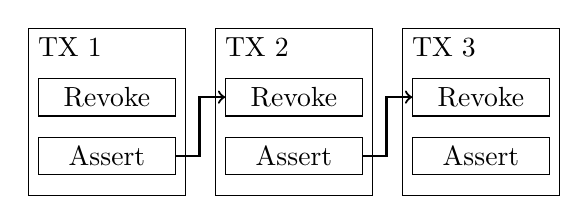
\begin{tikzpicture}
% \node at (-1, 2.5) {Inputs};
% \node at (5, 2.5) {Outputs};
\draw (0, 0.75) rectangle (2,2.875);
\node[below right] at (0, 2.875) {TX 1};
\node[draw, text width=1.5cm, align=center] (Revoke 1) at (1,2) {Revoke};
\node[draw, text width=1.5cm, align=center] (Assert 1) at (1,1.25) {Assert};

\draw (2.375, 0.75) rectangle (4.375,2.875);
\node[below right] at (2.375, 2.875) {TX 2};
\node[draw, text width=1.5cm, align=center] (Revoke 2) at (3.375,2) {Revoke};
\node[draw, text width=1.5cm, align=center] (Assert 2) at (3.375,1.25) {Assert};

\draw (4.75, 0.75) rectangle (6.75,2.875);
\node[below right] at (4.75, 2.875) {TX 3};
\node[draw, text width=1.5cm, align=center] (Revoke 3) at (5.75,2) {Revoke};
\node[draw, text width=1.5cm, align=center] (Assert 3) at (5.75,1.25) {Assert};

\draw[->, thick] (Assert 1) -| (2.175, 2) |- (Revoke 2);
\draw[->, thick] (Assert 2) -| (4.55, 2) |- (Revoke 3);

\end{tikzpicture}
\vspace*{4mm}
